\iffalse \bibliography{include/backmatter/magnus,include/backmatter/philip} \fi

\chapter{Introduction}
In order for organisations to remain competitive, there is a need to continuously improve time to market for new features and services. The societal transformation of moving from a product economy to a service economy has affected the way organisations deliver software \cite{mckinsey}. Cloud computing is a direct response to the need of agility and has increasingly earned the reputation of being the holy grail of application deployment \cite{7034713}. Products are required to move from business requirements to delivery as fast as possible. DevOps is a new development methodology which allow companies to stay competitive through enabling agility within the software release process. The aim of DevOps is to break the wall between developers and operations professionals in order to minimize deployment delays and to streamline the delivery process \cite{Httermann:2012:DD:2380958}. New tools and new methodologies that help automate the entire release process are required in order to pursue a successful delivery process.\\

Virtual Machines (VM) and Linux Containers are popular tools that are used to simplify application release processes, especially in Cloud computing. Virtual machines permit workloads to be isolated from one another and for resource usage to be somewhat controlled \cite{vmvscontainers}. Docker, a Linux container manager, is different from running an entire virtual machine in that it delivers systems or applications packaged into containers, instead of automating and making the deployment and management process as transparent and multi-platform as possible \cite{vmvscontainers}. Docker solves the same problem that faced the cargo industry; deliver goods in a standardized container so that any means of transport is capable of delivering the goods. A Dockerized application instance runs on top of a lightweight VM with a complete copy of the file system, “sand-boxed” from other Dockerized instances. Each change to the file system in a container acts similarly to how revision control systems such as git works. Starting from a base image, any subsequent change is stored on a new layer which in turn decreases subsequent build times and allows for safe roll-backs.\\

When having a complete system decomposed in multiple containers, responsibilities are isolated between each other during run-time, minimizing component dependencies. This allows development teams to work independently on each container with separate versioning. This avoids the big-bang integration approach and allows the possibility to carry out A/B testing for each separated component. Docker has been strongly adopted for web-applications, such as Twitter and eBay \cite{7034713}. Having software components containerized introduces performance overhead when compared to running the application natively, as identified in \cite{7034713}.\\

The question remains, how much performance overhead is introduced when using Docker, specifically when real-time requirements are mission critical? Failing to meet the real-time requirements for autonomous self-driving vehicles could lead to catastrophic effects. The software composed for self-driving vehicles could benefit by the use of virtualisation, during development (such as safe roll back and independent versioning) as well as post-development to ship updates and patches. In order to consider the use of virtualisation containers for real-time systems, one needs to first understand the overhead that is introduced by virtualisation to ensure that the systems meet the real-time requirements for the safety measures needed in an autonomous self-driving vehicles.\\

\section{Background}

The engineering challenge for this research is to identify the performance overhead when utilising lightweight virtual containers as part of the deployment pipeline for real-time systems. Current literature \cite{vmvscontainers} presents results on the performance overhead when utilising Docker and KVM. However, there exists a research gap in the contexts of real-time systems and how the utilization of software containers affects the performance of such systems. The results of this study will be used to identify the overhead costs of utilizing virtual environments, such as Docker, on standard and patched operating systems (Ubuntu and Ubuntu RT-Preempt) in the context of a real time system.\\

The paper presented by C. Berger \cite{cberger} presents the exploration of a deployment strategy in the context of self-driving vehicles that utilises lightweight Docker containers. However, the paper does not look to identify the precise performance overhead when using Docker as part of the deployment strategy. This paper aims to build on the research presented by C. Berger in order to fulfil a gap in current literature by identifying such performance-costs through exploring multiple software setups, configurations and system load. Prior research paper \cite{cberger} also addresses the need for future work being done within the topic of this research.\\

Current literature \cite{vmvscontainers} presents compelling evidence for the existence of performance overhead when running applications within a virtualised environment. This evidence is based on an exploration of Docker, KVM, and native environments without exploring the impact such environments have on time critical software. This further enhances the underlying need of understanding what delay-impact virtual containers have on time critical systems such as software for self-driving vehicles. Self driving vehicles require minimal delays during runtime to allow real-time computations to enable autonomous driving that is safe. Minimal time-delay is a fundamental concern for allowing lane-following, decision making, and other computations utilized by the autonomous vehicle to interact with its surroundings.\\

While this research bases its merits on a narrow field of interest, its application can be used for a broad audience within the research community as well as for organisations interested in adopting new technology to improve software deployment for real-time systems. As more segments of today's society are becoming automated and reliant on software decision making, real-time systems plays an integral part of this development. Financial, aviation, and vehicle systems are just a few examples of domains with systems that are highly sensitive to time delays. A self-driving vehicle has to interpret its surroundings in real-time where any delay can have a catastrophic effect. Similarly, applications in the financial domain have to react to market fluctuations within nanoseconds to avoid loss on investment.\\

\subsection{Docker}

Docker is an open source light-weight container environment which was initially launched in 2013 and has gained ground rapidly with its simplicity. The environment offered by Docker simplifies the process of software deployment by packaging all dependencies into a light-weight virtualisation container which ensures that all instances of the software is utilising the same dependent libraries. The functionality provided by Docker is comparable with virtual machines as both are virtualised environments where software applications can be executed with all dependent libraries and applications are installed. However, Docker, in contrast to virtual machines, is a light-weight alternative as it communicates directly to the host machine's kernel. A virtual machine has the additional level of a virtual operating system which adds complexity which does not directly speak with the host machine's kernel. With the benefit of packaging the dependent libraries and applications into the container, software developers can avoid uncertain deployments where library versions may differ between the developers' development environments and the live production environment. Docker presents further benefits such as safe roll-back between different software versions which provides projects' the ability to always be able to fall back on application versions which are known to function correctly. By providing these benefits project managers can feel secure in that there always exists a working runtime environment in the scenario of a new failing deployment.\\

The container in which Docker packages all dependent libraries and applications are referred to as a Docker image. This image contains everything which is required for an application to be executed. In the case of self-driving vehicles such dependencies may be image processing libraries such as OpenCV and the middle ware which enables the real-time application. When executing an application within Docker, a container is executed with based on the Docker image which consists of the installed libraries. This software design allows for split testing of software as the same application can be executed multiple times without clashing with the other contained application. Thus being optimal for testing different versions of the same application simultaneously while knowing there is no interference between the executed applications.\\

\subsection{Deployment strategy}

Software deployment is a crucial part of the software development, it refers to the activities which makes the software system available for use \cite{carzaniga1998characterization}. The process contains a number of activities which all play into the life cycle of a software system with the goal to implement into the runtime environment where the system is set to operate live. These activities are namely: \\

\textbf{Release} – is the activity of packaging the software for delivering it to the end user. This includes processes such as including the software's requirements and dependencies to external components, such as libraries and applications. It also includes the process of advertising – the process of informing interested parties about the software being released.\\
\textbf{Install} – refers to the activities of assembling all required resources for the runtime environment. It consists of two specific process, namely \textit{transfer} and \textit{configuration}. Where the former is the process of transferring the software from the developer to the runtime environment and the later is the process of making the software ready for activation.\\
\textbf{Activate} – is the process of executing the software and all dependent applications in the runtime environment.\\
\textbf{Deactivate} – is the opposite of the \textit{activate} activity.\\
\textbf{Update} – is the activity of updating the version of the running software which consists of similar activities of the \textit{install} activity.\\
\textbf{Adapt} – refers to the process of ensuring that the updated version is running correctly in the runtime environment.\\
\textbf{Deinstall} – is the activity of decommissioning the running software and includes sub-activities such as removing the external libraries and components.\\
\textbf{Derelease} – is the final activity which includes the process of advertising the withdrawal of the software system.\\

All these activities differ in how they are executed depending on the software engineering paradigm utilised for the software project. In traditional software engineering practices, e.g. the waterfall model, seeks to execute the software deployment process at the end of the software's development cycle. Whereas more novel software engineering practices aim to execute the software deployment process continuously throughout the software's development cycle. In state-of-art software engineering practices such as continuous integration and continuous deployment, requires software to be deployed daily \cite{meyer2014continuous}. Such requirements can easily make the process of software deployment exhausting and complex, where software tools such as Docker would simplify these processes greatly. Docker simplifies processes found within each of the software deployment activities, as it provides the runtime environment before the software deployment process has begun. The development environment is a clone of the production environment thus transferring the deployment processes from the live production server to a confined a secure location where the deployment process does not affect the usability of the current running software.\\


\begin{figure}[ht]
\centering
     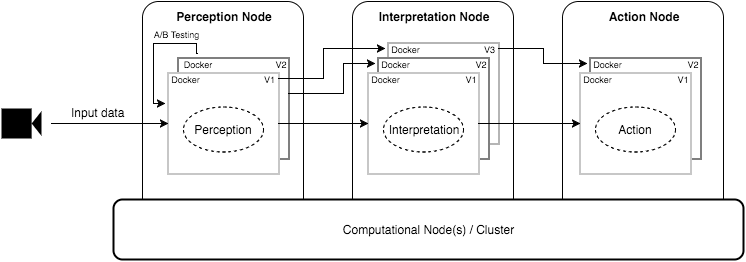
\includegraphics[width=1.0\textwidth]{./figure/containers.png}
      \caption{Run-time environment using Docker.}
       \label{containers}
\end{figure}

Figure \ref{containers} displays a deployment strategy design utilising Docker in the context of self-driving vehicles. The responsibilities are broken down into three computational nodes in which Docker containers are running instances of the code base independently. Each Docker container can run different versions of the separate nodes, where the interpretation node has three versions running separately. Version one (denoted V1) in each node represents the latest working configuration while other versions are run to test code which is still under development. Aforementioned, this allows for safe and simple roll-backs in the event of buggy code or degraded performance. Furthermore, multiple versioning of the same Docker container allows for split testing between different containers to take place. With an always functioning configuration, the development team can demonstrate the current status to stakeholders at any point in the development cycle. The ability to demonstrate the product at any point in the development phase adds to the business value as possible investors or stakeholders can see a functioning product even though it is currently under development. With current approaches this is possible, however it is not as straightforward and easily implemented as in cases which utilizes Docker for its deployment strategy.\\

\subsection{Kernel and CPU scheduler}

An operating system handles the communication between the software and the hardware, more specifically the operating system kernel acts as the interface between hardware and software. As an operating system is running a vast amount of processes simultaneously there is a need to prioritise and select which processes to run at what time. Each process utilises the CPU to make the computations required for the process to operate. The CPU is a powerful piece of hardware which can handle the same number of processes as it has cores and threads, i.e. an general Intel Core i7 processor has 4 cores and two threads per core amounting to 8 total processes simultaneously. However an operating system may run more processes than the CPU can process simultaneously. To manage this flood of processes a software component referred to as the \textit{CPU scheduler} which is configured by the kernel and is implemented to ensure that there is a queuing system set up for all processes running on the system. The \textit{CPU scheduler} acts as a traffic police in a busy intersection, handling a queue of all the processes running on the system by prioritising some processes ahead of other processes. The \textit{CPU scheduler} may act and prioritise differently depending on what rules have been set for it to follow.\\

The Linux OS CPU scheduler implements a FIFO (first-in-first-out) approach with two process scheduler algorithms, namely a time-sharing algorithm and a real-time algorithm. Where the former is a \textit{fair} scheduler algorithm trying to distribute the system's CPU resources equally over all processes in the queue ensuring that no process is completely starved. The later is an algorithm which prioritises the processes based on their set importance, where a higher prioritised process is provided more resources in comparison with a lower process. However, the generic Linux kernel version does not allow for any resource cut-off for processes utilising the CPU. A higher prioritised process will therefore not be able to utilise 100\% of the CPU's resources if there are other processes already using the CPU. This is not remarkable for a general purpose operating system running non-time sensitive applications. For a RT system it is crucial to ensure that the highest level process can interrupt any running processes at any point in time. An RT\_preempt kernel may be implemented to cope with such a design. This kernel design allows the scheduler to preempt any running process of lower priority than the requested process. Furthermore, the RT\_preempt kernel locks any resource utilised by a RT prioritised process.\\

\subsection{Middleware}



\subsection{Real-time systems and scheduling precision}

To understand the performance impact of utilizing Docker containers for the deployment strategy, the experiments of this research will analyse the scheduling precision of the automotive real-time application. The application executes computations within elements referred to as time-slices. The time-slice is a specification of time allocated for the algorithm to execute and deliver a result. A real-time application running at \texttt{100hz} executes 100 time-slices per second, which results in one time-slice being \texttt{10ms} or \texttt{0.01s}. The \texttt{10ms} time-slice is the time deadline set for the specific application, which is the maximum time allowed for the assigned algorithm to finish its computations. In scenarios where the algorithm utilizes less than the assigned time-slice the application will sleep for the remaining time until it fires a new execution. Assuring that the application sleeps for the specified time is a responsibility assigned to the operating system scheduler. Where the scheduler initiates processes which are sleeping and wishes to fire a new time-slice. Other than the assigned algorithm, the real-time application consists of code which is responsible for controlling the sleep of the time-slices. Therefore a part of the time-slice has to be consumed to execute the required code. The time consumed by the code which controls the sleep of the application is referred to as the OpenDaVINCI overhead which is part of what is used for measuring the scheduling precision of the execution environment.\\

Scheduling precision refers to how accurately the application executes the specified algorithm from the point of firing the time-slice until the algorithm begins its computation. Further accuracy is measured between the point of where the algorithm finishes its computations until the real-time application sleeps. Lastly, measurements are done to see whether the \texttt{sleep} function of the system actually sleeps for the remainder of the time-slice or if it overstays the specified time deadline.\\

The limitations of each execution environment can be identified by understanding how much time each part of the required code occupies the time-slice. The less time required for executing the code outside of the assigned algorithm the more deterministic a system is said to be. In a scenario where the assigned algorithm requires 80\% of the time-slice to execute the code, it is assumed that the application will sleep for the remaining 20\%. However, as there exists additional operations surrounding the algorithm the application might sleep 18\% whereas 2\% is required for the surrounding code to execute. If the application still sleeps 20\%, executes the algorithm for 80\%, and uses 2\% for the required code it will overstay its time-slice by 2\% thus rendering the application less deterministic. It is the time available for the algorithm the experiments will seek to identify to inform software engineers of how much of the time-slice can be used for effective computations, i.e. time available for generating a result.\\



\subsection{Disk IO and camera IO}

% \textit{Summary: This section will provide additional information on the RT\_PREEMPT Patch, OpenDaVINCI, Operating System Schedulers, what is means to be a deterministic and include terminology that readers may not be familiar with.}


\section{Problem Domain \& Motivation}
Our current society is increasingly depending upon real-time systems and automated solutions for many of the fundamental building blocks to the modern world. Such systems are used within financial, aviation, and automotive sectors. Sectors where these systems play an integral role in enabling automation to provide the services we all depend on today. With these industries advancing rapidly there is a need in understanding how software engineers should best work while developing the systems that drives the progress. With work, we specifically refer to the way the work flow of these software projects is structured in terms of integrating and deploying software. Where this research seeks to specifically answer the uncertainties that exists within the automotive industry. \\

There exists no evidence which presents argumentation on how state-of-art deployment strategies impact real-time systems within autonomous self-driving vehicles and their time sensitive performance requirements. Current literature \cite{vmvscontainers} explores the overhead for general purpose operating system in the context of cloud-computing, which differs in requirements from that of an autonomous self-driving vehicle's real-time system. This creates a compelling gap in literature to explore the field of automotive by building argumentation which decision makers can rely upon when determining for which strategy is most suitable for the real-time application in question. The popularity of deployment strategies utilising containers is steadily increasing, thus making it intriguing to understand the performance overhead introduced by containers such as Docker. While the implementation of virtualisation technologies for deployment strategies brings many advantages, there still exists uncertainty to the disadvantage of how much, if any, performance overhead they carry.\\

It is of particular importance to understand this impact for decision makers responsible for determining deployment strategies for time-critical systems utilized by self-driving vehicles. The rationale being that real-time systems are time constrained and must guarantee responses within a specified time deadline. If the system is to violate the specified deadline it may lead to software failure, which can potentially be catastrophic in the context of autonomous self-driving vehicles. Therefore it is crucial to ensure that the execution environment and deployment context will allow the real-time application to stay within its specified deadline. This is the gap in which the result of this research will seek to fulfil. Gaining specific measurement data of whether Docker carries extensive performance overhead will be an ultimate factor when deciding an approach to software deployment for real-time systems implemented in autonomous self-driving vehicles.\\

% What is the connection with deployment?
% check if the info in this section is really reflecting and following the reasoning you pitched in the previous subsections
\section{Research Goal \& Research Questions}
This research seeks to systematically study the impact of various execution contexts of two sample applications realised with OpenDaVINCI. The execution environment refers to the configuration of the target system including but not limited to system load, the deployment strategy and an alternation of a set of chosen Linux kernels. Methods of experimentation is used to answer the following research questions:\\

\begin{enumerate}[label=\textbf{RQ\arabic*}]
\label{section:rqs}
	\item Does the respective execution environment influence the scheduling precision of the respective application?
	\item Does the respective execution environment influence the input/output performance of the respective application?\\
\end{enumerate}



%This research seeks to systematically study the performance impact of using lightweight virtual containers as a deployment strategy for real-time systems in the context of autonomous self-driving vehicles. Data is collected by means of executing an application developed together with the open source development architecture for cyber-physical systems, OpenDaVINCI \cite{OpenDaVINCI}, which has been used to realise a number of self-driving vehicles. Methods of experimentation is used to answer the following research questions:


%By analysing data extracted from executions made in an application which is being implemented in vehicles today, we seek to find firm evidence which considers overhead introduced by code required for executing the real-time application (RQ1). Additional overhead may exist when executing the real-time application with other load bearing factors such as capturing images from a camera (writing and reading to disk). Thus making it important to understand how Docker affects the performance of the real-time application when including external components which are required in the development of a self-driving vehicle (RQ2).\\



\section{Contributions}
% \textit{Summary: The contribution made to the research community by answering the RQs.} 


\section{Scope}
% \textit{Summary: In this section we will introduce the scope which is self-driving vehicles. The hardware we are using is in-line with actual hardware used in autonomous vehicles. The software development architecture used for our experimental units have been adopted in research projects involving the actual development of autonomous vehicles. We do not aim for our results to be valid in other types of autonomous systems, such as drones. }

\section{Structure of the article}

% \textit{Summary: In this section we will introduce a typical outline of the paper.}


% information on:
	% RT Preempt Patch
	% OpenDaVINCI
	% Schedulers
	% Real Time Systems
		% Time-slice
	